%!TEX root = MS42.tex
\section{Projecting Issues}
In this section are described some of the major implementation problems encountered during the realization of the project and that unfortunately remained in part unresolved. When designing a controller, certainly one requirement that has to be met is to reach an efficient complexity in terms of computational resources. In the sequel it's analyzed a category of control strategies which requires, at least in this case study, the exploitation of a big amount of resources that unfortunately weren't available on the machines used for experiments. Another flaw encountered regards the process of switching from the simulation environment to the real robot interface. As expected, even if the robot has been modeled and rendered almost perfectly for the simulation purpose, it lacks some important aspects of its dynamics.
\subsection{Adaptive Control}
In the previous sections it has been assumed that the dynamic model of the robot is perfectly known at any instant of time, but, in practice, this can't be always true. In fact there exist some model uncertainties depending on the robot configuration, mainly mechanical parameters like inertia matrices and masses for the single links or those related to the robot payload. To overcome this intrinsic problem, it is always possible to write the dynamic model of the robot \eqref{eq:robotdynamics} through a linear parametrization
\begin{equation}
M(q)\ddot{q} + C(q,\dot{q})\dot{q} + g(q) = Y(q,\dot{q},\ddot{q})\pi = \tau
\end{equation}
where the vector $\pi\in\mathbb{R}^r$ contains the combinations of the aforementioned physical parameters and $Y(q,\dot{q},\ddot{q})\in\mathbb{R}^{n\times r}$ is called the \textit{regressor} matrix. In brief, this sums up the aim of the \textit{Adaptive Control}, which, as the name suggests, makes the control law to adapt to the variations of the unknown robot model parameters. Recently, an analytic closed formula for the regressor has been derived from the Lagrange equations, in terms of the Denavit-Hartenberg parameters and the joints configurations  $q,\dot{q},\ddot{q}$, and implemented in \textit{Mathematica} environment \cite{gabiccini09}. For a 7-links manipulator like KUKA LWR, the resulting regressor matrix has dimensions $7$x$70$ in its unsimplified form, making literally impossible to handle an adaptive control with the owned instruments.
\subsection{From Simulation to Real Robot}
The purpose of the development of robotics applications in a simulated environment is exactly to test and debug the software produced before loading it on the physical robot. Ideally, this passage would occur seamlessly (see \autoref{fig:rosgazebointeraction}), but for several reasons which are now explained it doesn't happen in reality.
\begin{figure}[t]
\centerline{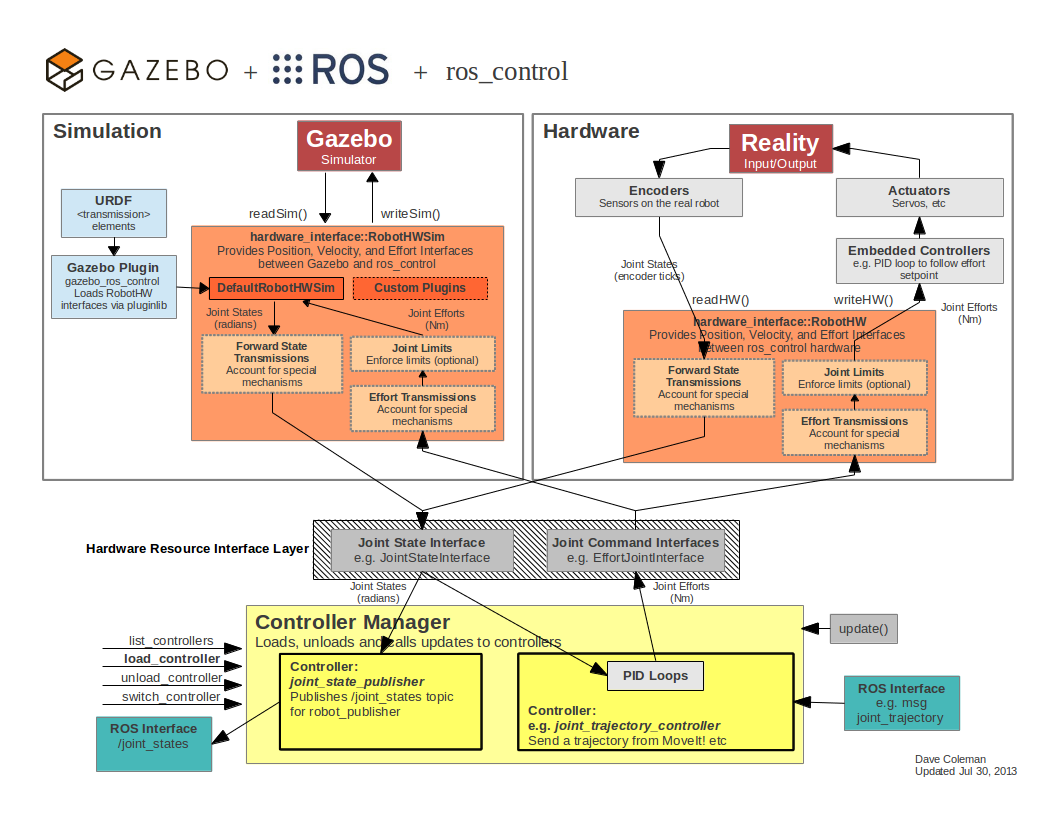
\includegraphics[scale=0.6]{ros+gazebo}}
\caption[Scheme of the interaction between ROS and Gazebo.]{Scheme of the interaction between ROS and Gazebo, with particulars on simulated and real robot.}
\label{fig:rosgazebointeraction}
\end{figure}
\subsubsection{Sensors Measurements}
The first discrepancy regards the presence of sensors for joint velocities measurements. In fact, while Gazebo provides them accurately through simulated sensors, the KUKA LWR arm is only equipped with position and torque sensors. This, indeed, arises the need to derive the velocities from the measured positions through a process of online differentiation, with the following methods being analyzed
\paragraph{Euler Method}
This is one of the most basic techniques to compute numerical differentiation and its formulation is
\begin{equation}
\dot{q}_n = \frac{q_n - q_{n-1}}{h}
\end{equation}
where $h$ is the sampling time. Since the output of this differentiator is usually a bit noisy, it's convenient to pass it through an exponential smoothing filter, which is basically a weighted average between the last computed velocity value and the previous one
\begin{equation}
\tilde{\dot{q}}_n = \alpha\dot{q}_n + (1-\alpha)\tilde{\dot{q}}_{n-1} 
\end{equation}
where $\tilde{\dot{q}}$ denotes the smoothed value and $\alpha\in(0,1)$ is the smoothing factor.
\paragraph{Levant Robust Differentiator}
This method is based on the sliding mode theory and gives asymptotically exact derivatives \cite{levant06}. In comparison with Euler, Levant differentiator performs significantly better in terms of noise rejection and derivation of signals, but the major flaw which led this method to be discarded is that introduces a relevant phase shift.\\[1em]
So, according to the tests conducted and evaluating a trade-off between exact but out-of-phase signals and noisy but coherent signals, the best method resulted the Euler one.
\subsubsection{Gravity Compensation}
Recalling the built-in controllers \eqref{eq:cartesianstiffnesscontroller},\eqref{eq:axisspecificstiffnesscontroller} of the KUKA LWR arm, the term $f_{dynamics}(q,\dot{q},\ddot{q})$ must be analyzed. It refers to the gravity compensation performed internally by the robot, in a way that the commanded torque isn't indeed affected by the gravitational field. This, unfortunately, generates a conflict between the internal compensation and the whole control law, which at dynamic level requires the knowledge of the gravitational force to compute the input torques. Since such term can't be forced to zero, one workaround could be that of not considering the gravity ($g(q)=0$) in all model-based controller, introducing a really negligible error.
\newpage